\clearpage
\chapter{PROPOSED WORK AND METHODOLOGY}
\section{Current Architecture}
The existing architecture of the Namaste BHU application is straightforward, comprises a comprehensive framework that encompasses web server components, a mobile application interface, a centralized database, and integration with Firebase for notifications. This architecture is designed to provide a seamless and user-friendly experience for students, faculty, and staff at Banaras Hindu University (BHU).

\begin{figure}[h]
    \centering
    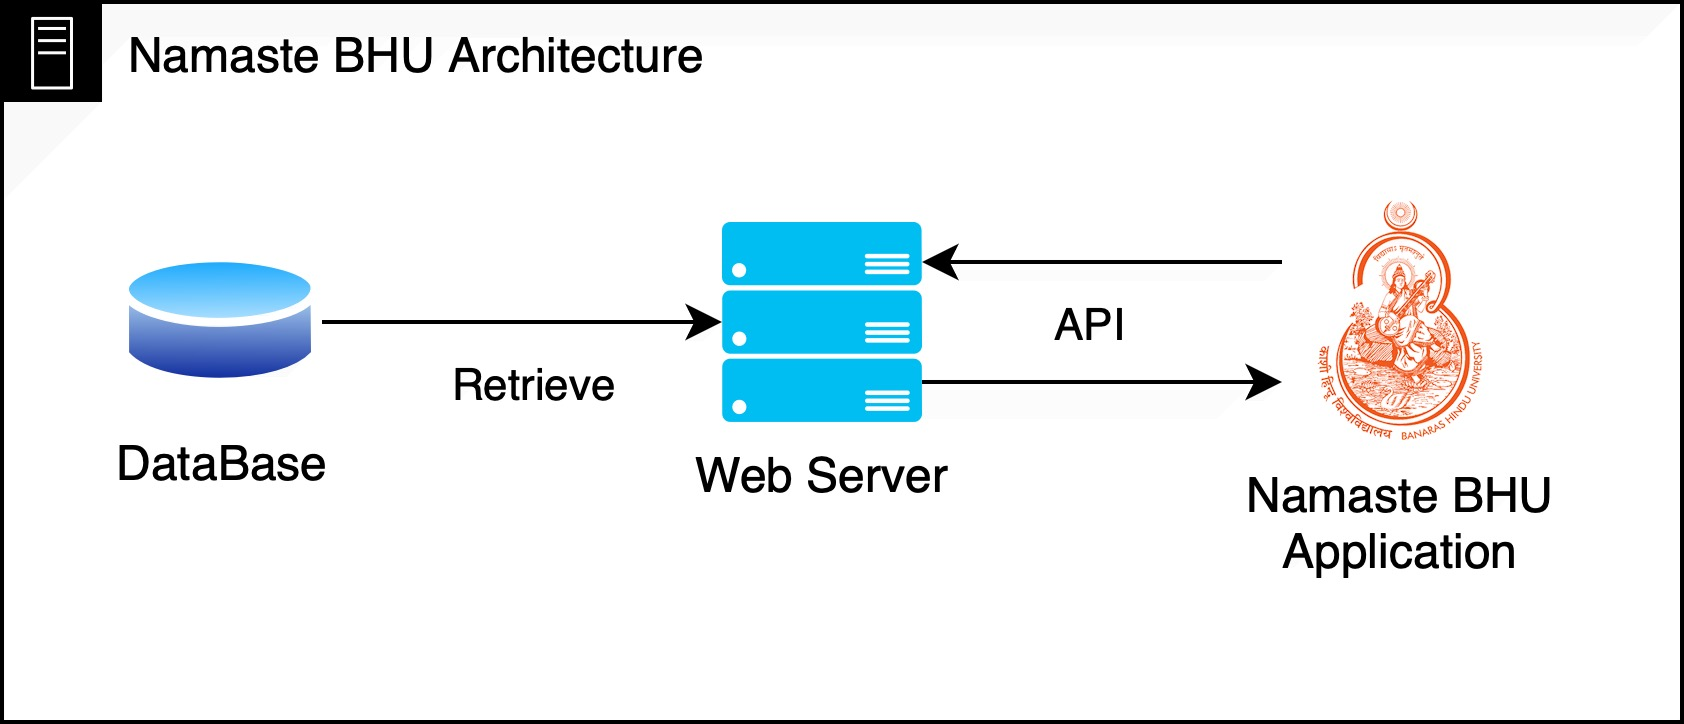
\includegraphics[width=0.75\linewidth]{assets/img/namaste-arch.jpg}
    \caption{Namaste BHU Architecture}
    \label{fig:namaste-arch}
\end{figure}

\textbf{Web Server}\\
The Namaste BHU web server components form the backbone of the application, serving as the centralized hub for managing and delivering various features and functionalities. The web server facilitates the exchange of data between the client-side interfaces (web and mobile) and the backend database, ensuring real-time updates and synchronization of information.

\textbf{Mobile Application}\\
The Namaste BHU mobile application serves as the primary access point for users to interact with the application on their mobile devices. It provides a user-friendly interface that enables students, faculty, and staff to access course materials, receive notifications, view event schedules, and engage with other features of the platform.

\textbf{Database}\\
The centralized database forms the core repository of data for the Namaste BHU application, housing essential information related to courses, students, faculty, events, and administrative records.

\section{Possible Solutions}
The integration of an LMS with the existing architecture of the Namaste BHU application presents a significant opportunity to enhance the academic experience and administrative efficiency within Banaras Hindu University (BHU). Several possible solutions can be considered to achieve this integration, each with its unique advantages and considerations. The following outlines some of the potential approaches:

\subsection{Development of a Custom LMS}
One possible solution involves developing a custom Learning Management System (LMS) specifically tailored to the needs and requirements of Banaras Hindu University (BHU). This approach offers the advantage of creating a bespoke solution that seamlessly integrates with the existing Namaste BHU architecture, providing a cohesive and unified platform for managing academic activities.

\subsection{Integrating an existing LMS}
Another possible solution is to integrate an existing Learning Management System (LMS) with Namaste BHU, leveraging the capabilities and features of established LMS platforms to enhance the academic experience and administrative efficiency within the university.

\begin{table}[h]
    \centering
    \begin{tabular}{|p{0.14\textwidth}|p{.38\textwidth}|p{0.38\textwidth}|}
        \hline
        \textbf{Solution} & Development of a Custom LMS & Integrating an existing LMS \\
        \hline
        \textbf{Advantages} &
        \begin{itemize}[noitemsep,topsep=0pt,leftmargin=*]
            \item Tailored to BHU's specific needs
            \item Seamless integration with Namaste BHU
            \item Flexibility and Scalability
        \end{itemize} &
        \begin{itemize}[noitemsep,topsep=0pt,leftmargin=*]
            \item Ready-made solution
            \item Continuous updates and improvements
        \end{itemize}\\
        \hline
        \textbf{Challenges} &
        \begin{itemize}[noitemsep,topsep=0pt,leftmargin=*]
            \item Time and resources
            \item Technical complexity
            \item Maintenance and support
        \end{itemize} &
        \begin{itemize}[noitemsep,topsep=0pt,leftmargin=*]
            \item Compatibility and customization
            \item Training and user adoption
        \end{itemize}\\
        \hline
    \end{tabular}
    \caption{Comparing Approaches}
    \label{tab:approaches}
\end{table}

The above approaches to integrate LMS with Namaste BHU are summarized in the table \ref{tab:approaches} with their advantages and challenges. After careful consideration of various options for integrating a Learning Management System (LMS) with Namaste BHU, the solution to integrate an existing LMS was more feasible and Moodle, an open source LMS emerges as the preferred choice.


\section{Why Moodle?}
Moodle, an open-source LMS widely adopted in educational institutions worldwide, offers a robust set of features, flexibility, scalability, and a vibrant community of developers and users. The following factors contribute to the selection of Moodle for integration with Namaste BHU:

\begin{enumerate}
    \item \textbf{Open Source Platform}: Moodle is an open-source Learning Management System, providing flexibility, customization, and community support without the need for costly licensing fees.
    \item \textbf{Robust Feature Set}: Moodle offers a comprehensive set of features for course management, assessment, communication, collaboration, and reporting, catering to the diverse needs of educational institutions.
    \item \textbf{Scalability and Customization}: Moodle is highly scalable and can accommodate the growth of Banaras Hindu University's user base, courses, and content over time. Moodle allows for extensive customization through plugins, themes, and modules, enabling tailored solutions to meet BHU's specific requirements and preferences.
    \item \textbf{Integration Capabilities}: Moodle offers seamless integration with third-party systems and services, facilitating integration with Namaste BHU and other university applications.
    \item \textbf{Active Community}: Moodle boasts a vibrant and active community of developers, educators, and administrators who contribute to ongoing development, support, and innovation.
\end{enumerate}

\section{Moodle Architecture}
Moodle follows a modular architecture that comprises several key components working together to deliver its functionality. Moodle's architecture consists of several key components that work together to provide a flexible, scalable, and customizable learning management system. The following components form the foundation of Moodle's architecture:

\begin{figure}[h]
    \centering
    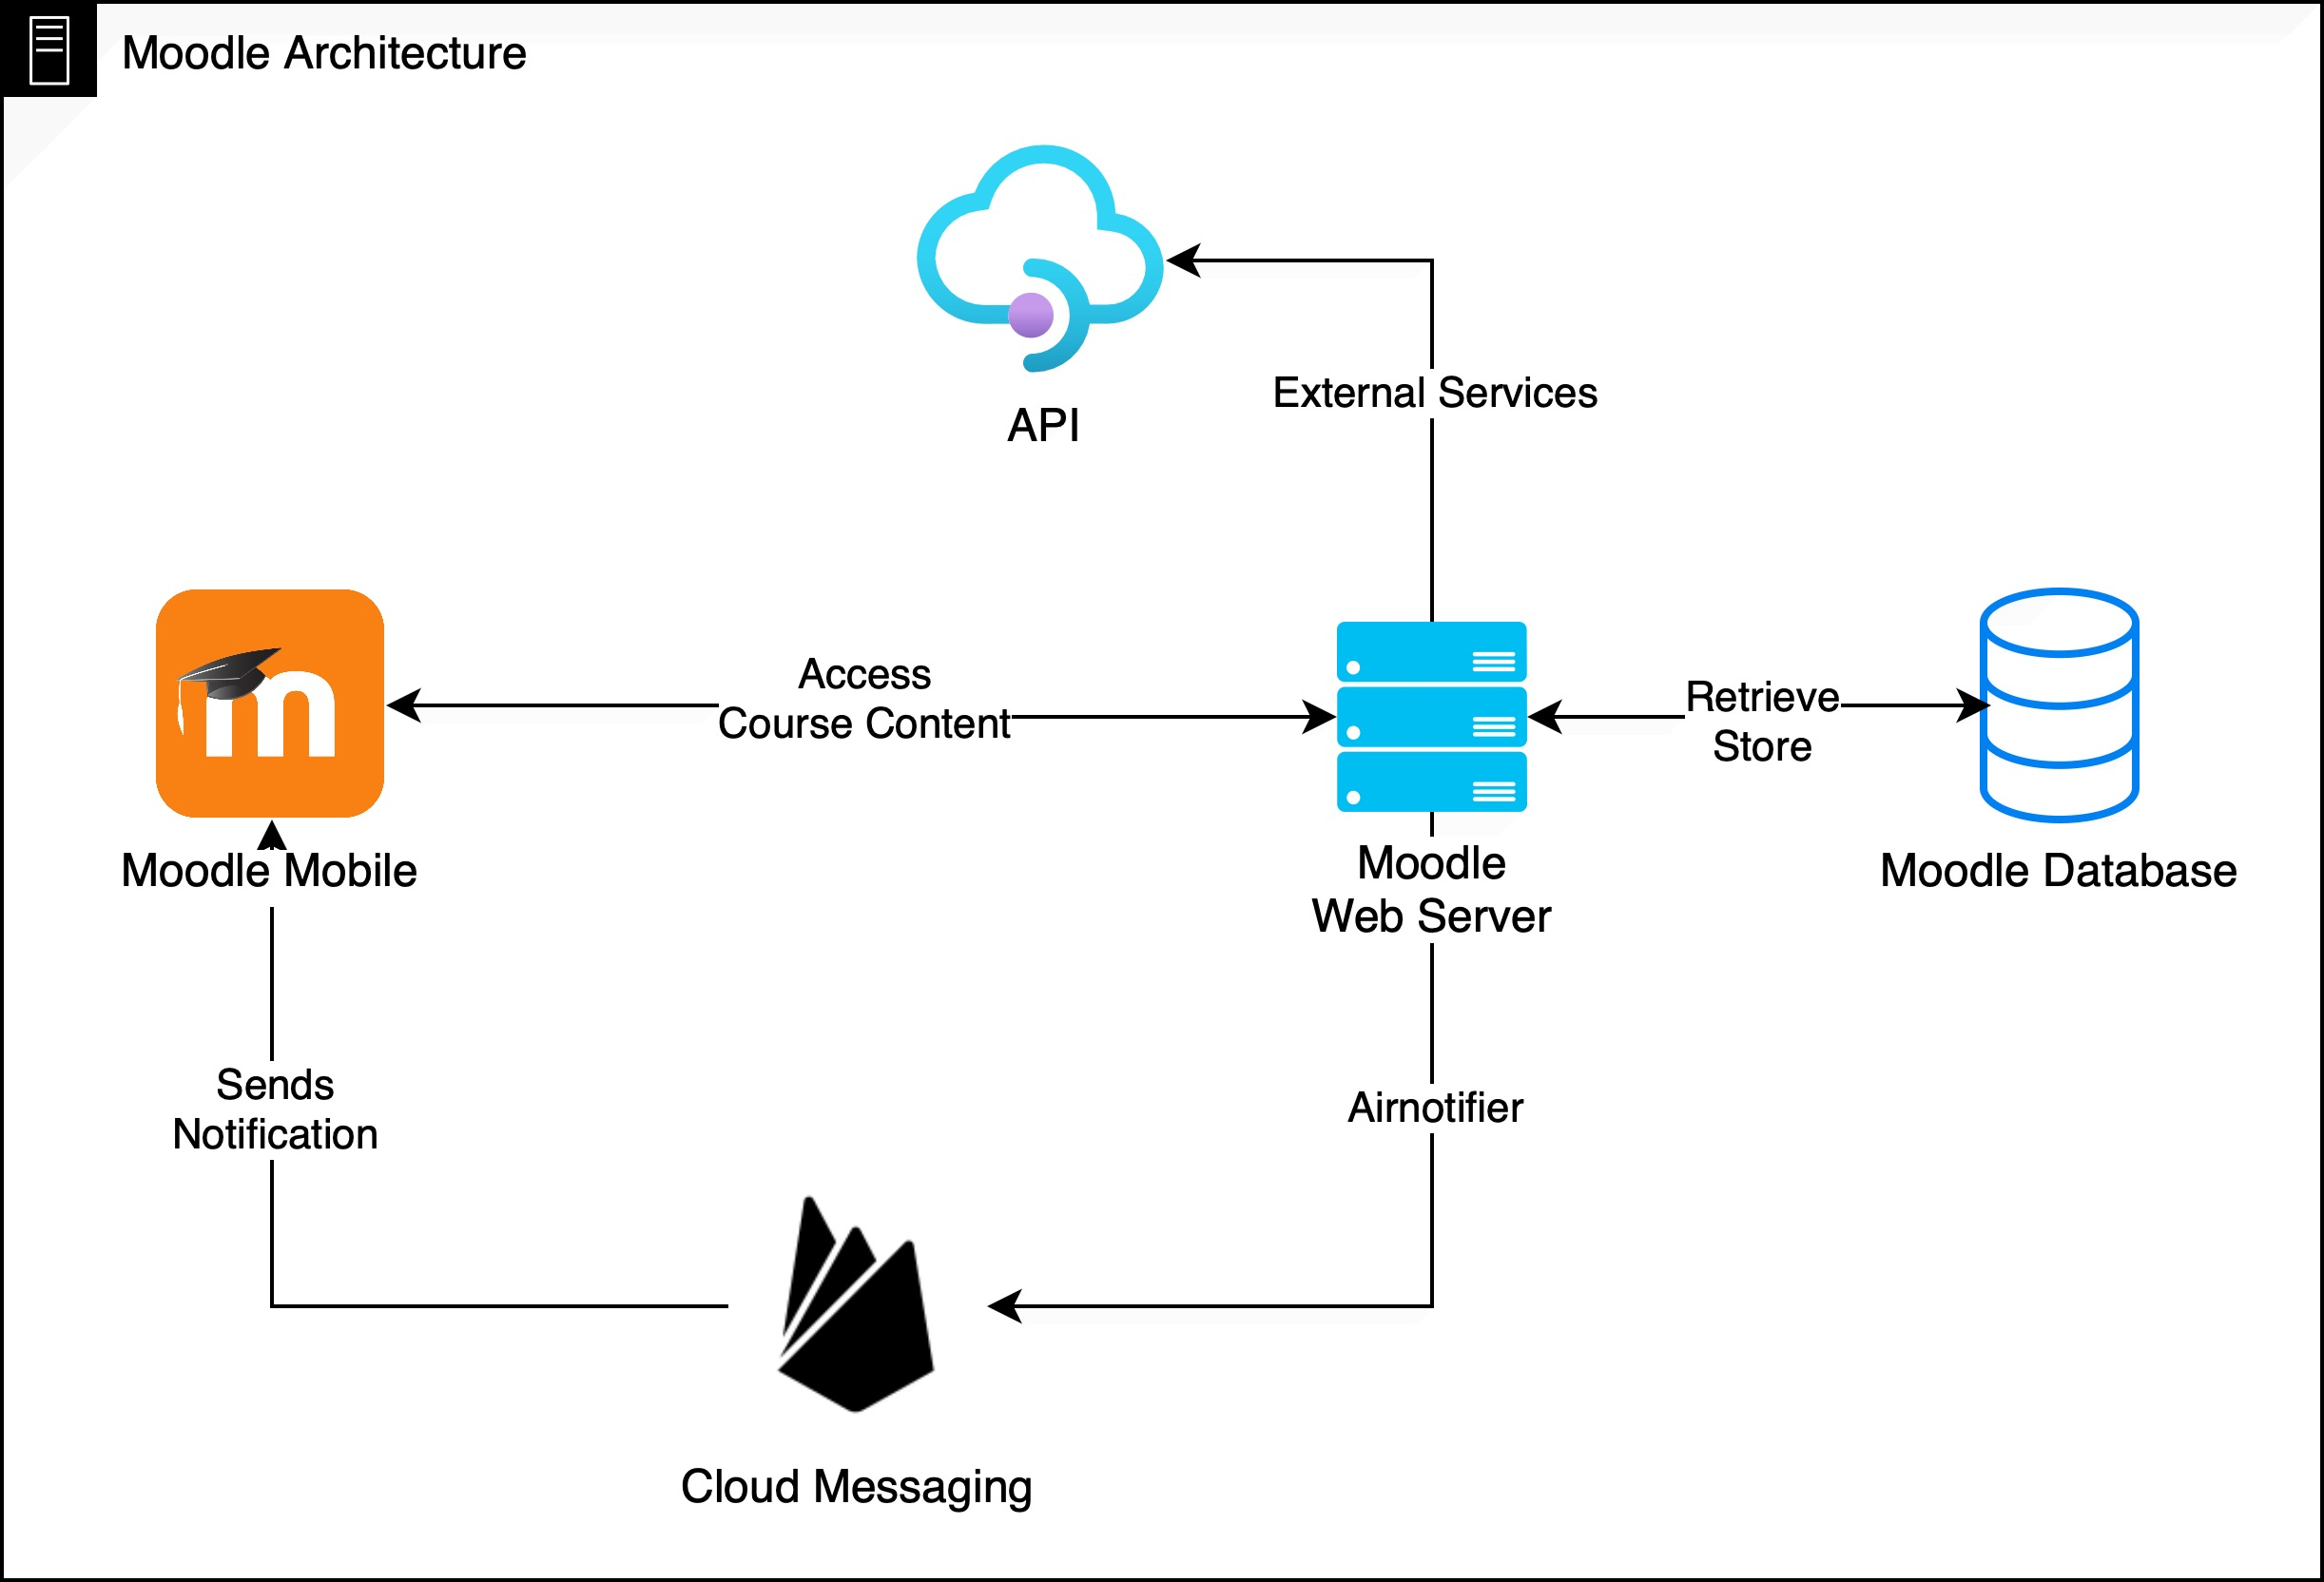
\includegraphics[width=0.75\linewidth]{assets/img/moodle-arch.jpg}
    \caption{Moodle Architecture}
    \label{fig:moodle-arch}
\end{figure}

\textbf{Web Server}\\
The web server component serves as the central point of access for users to interact with Moodle. It hosts the Moodle application and delivers web-based content, interfaces, and services to users across different devices and platforms.

\textbf{Moodle Mobile}\\
Moodle Mobile is a companion application that extends the functionality of Moodle to mobile devices, including smartphones and tablets. It provides users with access to course materials, activities, and communication tools on the go, enabling anytime, anywhere learning.

\textbf{Database}\\
The database component of Moodle stores and manages essential data related to courses, users, activities, resources, grades, and other aspects of the learning environment. Moodle supports multiple database management systems (DBMS), including MySQL, PostgreSQL, and Microsoft SQL Server, allowing for flexibility in deployment and scalability.

\textbf{Plugins}\\
Plugins are modular extensions that enhance the functionality and features of Moodle. They can be installed, enabled, and configured to add new capabilities, such as activity modules, resource types, authentication methods, themes, and blocks. Moodle's plugin architecture allows for easy customization and extensibility to meet specific user needs and requirements.

\textbf{APIs (Application Programming Interfaces)}\\
Moodle provides a set of APIs that enable integration with external systems, services, and applications. These APIs allow developers to interact with Moodle programmatically, access and manipulate data, and perform various operations, such as user authentication, course enrollment, content management, and activity tracking. Moodle's APIs support standards such as REST (Representational State Transfer) and XML-RPC (Remote Procedure Call), facilitating interoperability and integration with third-party platforms and tools.


\section{Proposed Architecture}

The proposed architecture for integrating Moodle with the Namaste BHU application entails maintaining both environments separately while facilitating seamless communication and data exchange between them. This approach leverages the strengths of both systems to provide an enhanced academic experience for students, faculty, and staff at Banaras Hindu University. The key components of the proposed architecture are as follows:

\textbf{Separate Environments}\\
The integration involves maintaining Namaste BHU and Moodle as separate environments, each serving distinct purposes within the university ecosystem. Namaste BHU continues to function as the primary platform for campus life management, communication, and information dissemination, while Moodle serves as the dedicated learning management system for course delivery and academic activities.

\begin{figure}[h]
    \centering
    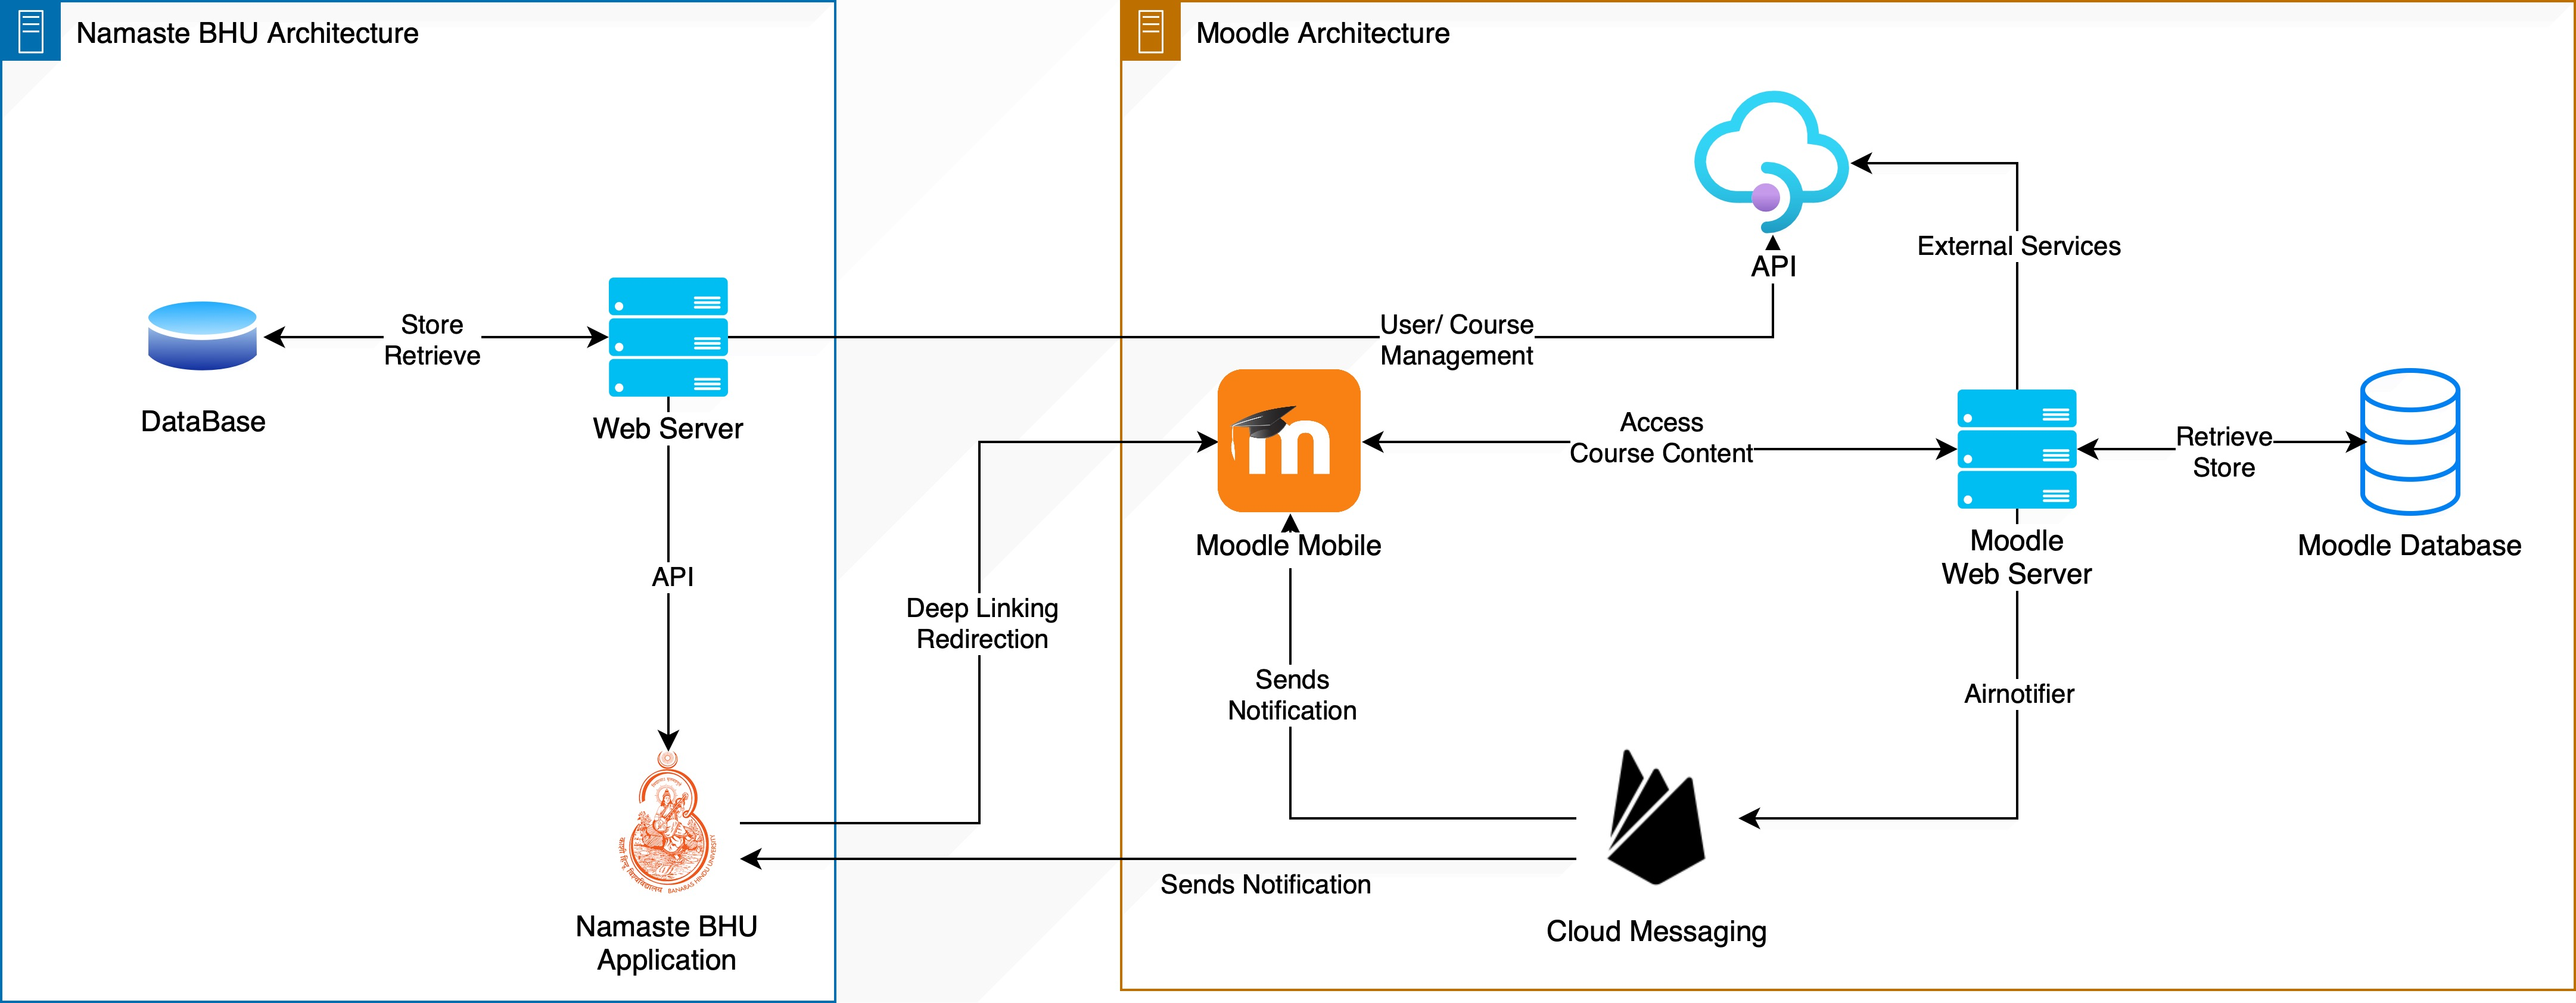
\includegraphics[width=\linewidth]{assets/img/proposed-arch.jpg}
    \caption{Proposed Architecture}
    \label{fig:proposed-arch}
\end{figure}

\textbf{Namaste Database Configuration}\\
The Namaste BHU database is configured to incorporate identifiers for courses, users, and access tokens required for seamless integration with Moodle. This involves updating the database schema to include fields for course IDs, user IDs, and authentication tokens, which facilitate the exchange of data between Namaste BHU and Moodle through APIs.

\textbf{Integration with Moodle APIs}\\
Moodle's APIs are utilized to establish communication between Namaste BHU and Moodle, enabling the exchange of data and functionalities between the two systems. Namaste BHU interacts with Moodle's APIs to retrieve course information, enroll users, synchronize content, and authenticate users seamlessly across both platforms.\\

\textbf{Moodle Web and Mobile Applications}\\
Users access Moodle's web and mobile applications to engage with course materials, activities, and resources offered through the integrated platform. Moodle's web application provides a comprehensive interface for accessing courses, participating in activities, and interacting with instructors and peers. The Moodle Mobile application extends the accessibility of Moodle to mobile devices, allowing users to learn on the go and stay connected with their academic progress.

\textbf{Seamless User Experience}\\
The proposed architecture aims to deliver a seamless user experience by integrating Namaste BHU's features and functionalities with Moodle's course management capabilities. Users can access course materials, receive notifications, participate in discussions, submit assignments, and view grades seamlessly across both platforms, enhancing their overall academic experience at Banaras Hindu University.
